\chapter{Methodology}

\section{Task}
For a short text segment, $T = \{t_1, t_2, ..., t_n\}$ where $t_i$ is defined as a token, classify if the sequence of tokens $T$ is a complaint or not.

\section{Data and pre-processing}
The data used for the experiments is from Twitter which provides a good representation of social media text due to the direct connection consumers have with organisations and brands \cite{preotiuc-pietro_automatically_2019}. With Twitter, users have a medium where they can self-express to a higher degree while maintaining flexible connections across their social network \cite{shane-simpsonWhyCollegeStudents2018}. The data set created by \cite{preotiuc-pietro_automatically_2019} and further used by \cite{jin_complaint_2020} is utilised for this project. The original process for collection and annotation employed by them is briefly described below. The particular version\footnote{\url{https://archive.org/details/complaint_severity_data}} used for the experiments is the one enhanced by \cite{jinModelingSeverityComplaints2021} with the addition of labels for the severity of complaints. These additional labels are not used for the experiments in this project.
\subsection{Criteria for tweets}
A cross-industry representative collection of 93 customer service handles of organisations on Twitter were identified manually. These handles were then categorised into 9 domains using their industry type. Since an organisation could have business activities across domains, the assigned domain was based on the products or services receiving the most number of complaints. All the domains used in the experiments are listed in Table \ref{tab: domains}.
\begin{table}[ht]
    \captionsetup{font=small}
    \small
    \centering
    \begin{tabularx}{\textwidth}{|X|c|c|c|}
        \hline
        \rowcolor[gray]{0.7}
        \textbf{Domains}            & \textbf{Complaints} & \textbf{Non-Complaints} & \textbf{Total Tweets} \\
        \hline
        Food \& Beverage            & 95 \small{(73\%)}   & 35 \small{(27\%)}       & 130 \small{(7\%)}     \\
        \rowcolor[gray]{0.9}
        Apparel                     & 141 \small{(55\%)}  & 117 \small{(45\%)}      & 258 \small{(13\%)}    \\
        Retail                      & 124 \small{(62\%)}  & 75 \small{(38\%)}       & 199 \small{(10\%)}    \\
        \rowcolor[gray]{0.9}
        Cars                        & 67 \small{(73\%)}   & 25 \small{(27\%)}       & 92 \small{(4\%)}      \\
        Services                    & 207 \small{(61\%)}  & 130 \small{(39\%)}      & 337 \small{(17\%)}    \\
        \rowcolor[gray]{0.9}
        Software \& Online Services & 189 \small{(65\%)}  & 103 \small{(35\%)}      & 292 \small{(15\%)}    \\
        Transport                   & 139 \small{(56\%)}  & 109 \small{(44\%)}      & 248 \small{(12\%)}    \\
        \rowcolor[gray]{0.9}
        Electronics                 & 174 \small{(61\%)}  & 112 \small{(39\%)}      & 286 \small{(15\%)}    \\
        Other                       & 96 \small{(79\%)}   & 33 \small{(21\%)}       & 129 \small{(7\%)}     \\
        \hline
        \rowcolor[gray]{0.9}
        \textbf{Total}              & 1232 \small{(63\%)} & 739 \small{(37\%)}      & 1971                  \\
        \hline
    \end{tabularx}
    \caption{The nine domains and the distribution of tweets that are complaints and those that are not. The percentages indicate how the splits are distributed \cite{preotiuc-pietro_automatically_2019}.}
    \label{tab: domains}
\end{table}

\subsection{Data Extraction}
Twitter API\footnote{\url{https://developer.twitter.com/en}} was utilised to extract the tweets. The latest 3,200 tweets at the time of the collection exercise were retrieved and the original tweets to which the customer service handles responded were identified. Random sampling equally for each handle, 1,971 tweets were then identified where there was a response from the support's handle. To ensure a more balanced and diverse dataset, 1,478 randomly sampled tweets were added to the dataset. 739 tweets were replies to other handles (outside the 93 identified) and the remaining 739 tweets were not addressed to any Twitter handle. Table \ref{tab: tweet_counts} shows the breakdown of the total population of the tweets dataset. Tweets were filtered for English using langid.py \cite{luiLangidPyOfftheshelf2012}. Retweets were excluded and all usernames and URLs were anonymised and replaced with placeholder tokens.
\begin{table}[ht]
    \captionsetup{font=small}
    \small
    \centering
    \begin{tabularx}{\textwidth}{|X|c|c|c|}
        \hline
        \rowcolor[gray]{0.7}
        \textbf{Extraction Criteria}                                           & \textbf{Complaints} & \textbf{Non-Complaints} & \textbf{Total Tweets} \\
        \hline
        Addressed to and replied by the identified 93 customer service handles & 1239 \small{(63\%)} & 739 \small{(37\%)}      & 1971 \small{(58\%)}   \\
        \rowcolor[gray]{0.9}
        Addressed to other customer service handles                            & 0                   & 739 \small{(100\%)}     & 739 \small{(21\%)}    \\
        Not addressed to any Twitter handle                                    & 0                   & 739 \small{(100\%)}     & 739 \small{(21\%)}    \\
        \hline
        \rowcolor[gray]{0.9}
        Total                                                                  & 1232 \small{(36\%)} & 2217 \small{(64\%)}     & 3449                  \\
        \hline
    \end{tabularx}
    \caption{Selection of tweets based on random sampling and where they have received replies when addressed to the 93 customer service handles combined with random sampled tweets that are addressed to other handles (random\_reply) and tweets that are not addressed to any handle (random\_tweet) \cite{preotiuc-pietro_automatically_2019}.}
    \label{tab: tweet_counts}
\end{table}

\subsection{Annotation}
The classification of the 1,971 tweets as complaints or not was carried out using a binary annotation task (complaint or not). Since tweets are concise and typically express a single idea, an entire tweet was classified as a complaint if it contained at least one speech act of complaining. To guide the annotation process, a complaint definition from \cite{olshtain_speechact_1987}, stating that a complaint portrays a situation that contradicts the writer's positive expectation was used. Two of the authors with extensive annotation experience in linguistics independently labelled the 1,971 tweets. They had substantial agreement \cite{artsteinInterCoderAgreementComputational2008} with Cohen's Kappa of $\kappa$ = 0.731. In the end, 1,232 tweets (63\%) and 739 tweets (37\%) were identified as complaints and non-complaints. Table \ref{tab: domains} gives the breakdown of the complaint and non-complaint tweets for each domain.

\section{Environment}

The key details of the environment used for the experiments are listed below. All experiments are run in a Jupyter Notebook and on a single GPU.
\subsection{Hardware}
\begin{itemize}
    \small
    \item \textbf{CPU Count:} 8
    \item \textbf{System Memory:} 45 GB
    \item \textbf{GPU Count:} 1
    \item \textbf{GPU Model:} NVIDIA RTX A4000\footnote{\url{https://www.nvidia.com/en-gb/design-visualization/rtx-a4000/}}
    \item \textbf{GPU Memory:} 16 GB
\end{itemize}

\subsection{Software}
For the experiments, the BERT large language model along with a number of its variants are used to classify the tweets and compare the performance. The models are based on the \texttt{transformers} library implementation from Hugging Face\footnote{\url{https://huggingface.co/}} \cite{wolfHuggingFaceTransformersStateoftheart2020} in Python. Additionally, the \texttt{datasets} and \texttt{evaluate} libraries are used. From scikit-learn\footnote{\url{https://scikit-learn.org/stable/}} the \texttt{sklearn} library is utilised to generate the stratified splits for the nested cross-fold validation. The versions for each library are shown in Table \ref{tab: libs_used}. The version of Python used is v3.9.16.

\begin{table}[ht]
    \captionsetup{font=small}
    \small
    \centering
    \begin{tabularx}{\textwidth}{|X|X|X|}
        \hline
        \rowcolor[gray]{0.7}
        \multirow{-3}{*}{} \textbf{Provider} & \textbf{Library Name} & \textbf{Version} \\
        \hline
        \multirow{3}{*}{Hugging Face}        & transformers          & 4.21.3           \\
        \cline{2-3}
                                             & datasets              & 2.4.0            \\
        \cline{2-3}
                                             & evaluate              & 0.4.0            \\
        \hline
        Scikit-Learn                         & sklearn               & 1.1.2            \\
        \hline
        Numpy                                & numpy                 & 1.23.4           \\
        \hline
        Pandas                               & pandas                & 1.5.0            \\
        \hline
    \end{tabularx}
    \caption{Software and library versions used for this project.}
    \label{tab: libs_used}
\end{table}

\section{Model selection}
The performance of BERT and its variants on the text classification task will be explored as part of the experiments. BERT \cite{devlinBERTPretrainingDeep2018} is based on the modern transformers network architecture \cite{vaswaniAttentionAllYou2023a}. Using BERT for the text classification task has several advantages over previous dominant methods such as Gated Recurrent Units GRU) \cite{chungEmpiricalEvaluationGated2014} or Long Short Term Memory (LSTM) \cite{hochreiterLongShortTermMemory1997} networks. Although tweets tend to be made up of short texts, the ability to capture long-term dependencies is still useful for understanding relationships across the content better. They also rely on bidirectional processing to use contextual information to have a more nuanced understanding of the intention of the author of the tweet or post. Since BERT is already pre-trained on large corpora, it is considered to possess a significant general understanding of the English language. Finally, the pre-training enables transfer learning and domain adaptation with relative ease which is very useful for tasks where annotated data is limited (only 3,449 tweets are used for the experiments).
\newline\newline
The transformer models used are listed in Table \ref{tab: model_dtls} along with the number of parameters for each of them. The number of parameters or model size is based on the embedding and output layers along with the attention heads. The models chosen are such that there is a wide range of model sizes, from RoBERTa Base and BERT Base with 125 and 110 million parameters to lightweight variants such as DistilBERT Base and BERT Tiny with much lower model sizes. This allows for a comparison of the model performance both in terms of the predictions as well as the inference time to the model size. Various studies have pointed to a relation between the size of the model and its predictive performance conditional to appropriate pre-training \cite{vaswaniAttentionAllYou2023a,liuRoBERTaRobustlyOptimized2019}. The summary of BERT Base and BERT Tiny are shown in Figure \ref{fig: model_summary} for a high-level perspective on the layers and the number of parameters in each of them.

\begin{table}[ht]
    \captionsetup{font=small}
    \small
    \centering
    \begin{tabularx}{\textwidth}{|l|X|l|X|}
        \hline
        \rowcolor[gray]{0.7}
        \textbf{Model}            & \textbf{Parameter Count} & \textbf{Tokenizer Type}  & \textbf{Vocab. Size} \\
        \hline
        RoBERTa Base              & 125M                     & Byte-level BPE           & 50,265               \\
        \rowcolor[gray]{0.9}
        BERT Base (uncased)       & 110M                     & WordPiece                & 30,522               \\
        BERTweet Base             & 110M                     & Byte-Pair Encoding (BPE) & 64,000               \\
        \rowcolor[gray]{0.9}
        DistilBERT Base (uncased) & 66M                      & WordPiece                & 30,522               \\
        ALBERT Base v2            & 11M                      & SentencePiece            & 30,000               \\
        \rowcolor[gray]{0.9}
        BERT Tiny                 & 4.4M                     & WordPiece                & 30,522               \\
        \hline
    \end{tabularx}
    \caption{The transformer models used for the experiments along with the type of tokenization, and vocabulary size and sorted by the number of parameters for each of them. The parameter counts are from \cite{bhargavaGeneralizationNLIWays2021} for RoBERTa Base, BERT Base, ALBERT Base and BERT Tiny. For BERTweet it is from \cite{nguyenBERTweetPretrainedLanguage2020}, and DistilBERT from \cite{sanhDistilBERTDistilledVersion2020}. Vocabulary sizes and tokenizer types are based on documentation at \texttt{https://huggingface.co/}.}
    \label{tab: model_dtls}
\end{table}

\begin{figure}[htb]
    \centering
    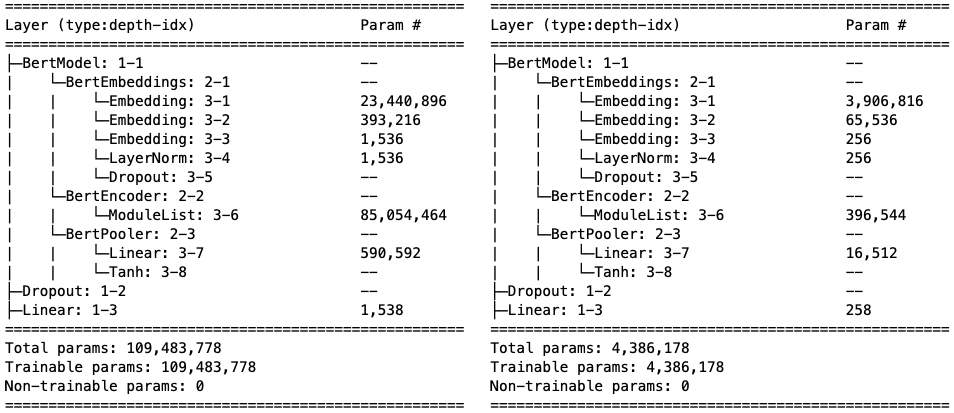
\includegraphics[width=15cm]{figures/model-summary.png}
    \vspace*{-3mm}
    \caption{A summary of the BERT Base (left) and BERT Tiny (right) models for comparison in terms of the layers used and number of parameters. This is based on the models from Hugging Face.}
    \label{fig: model_summary}
\end{figure}

\section{Data tokenisation}
The tokenization process is required for appropriate preparation of input data for use by BERT and its variants. The tokenization process\footnote{\url{https://huggingface.co/docs/datasets/use_dataset}} involves dividing the input text into tokens based on a predefined set of rules. These tokens are subsequently transformed into numerical representations and tensors, along with any extra inputs needed by the model. Tokens in general could be words, subwords, phrases or even characters. There are various approaches to tokenization and the methods used by each of the models in the scope of the experiments are indicated in Table \ref{tab: model_dtls}. The \texttt{transformers} library provides relevant methods to tokenize the input tweets. The library includes model-specific tokenizers such as, \texttt{BertTokenizer}\footnote{\url{https://huggingface.co/docs/transformers/v4.21.3/en/model_doc/bert#transformers.BertTokenizer}} or \texttt{RobertaTokenizer}\footnote{\url{https://huggingface.co/docs/transformers/v4.21.3/en/model_doc/roberta#transformers.RobertaTokenizer}} while models like BERT-tiny leverage existing ones. For the experiments, the \texttt{AutoTokenizer}\footnote{\url{https://huggingface.co/docs/transformers/v4.21.3/en/model_doc/auto#transformers.AutoTokenizer}} has been used which conveniently selects the appropriate tokenizer relevant for the model in use.

\subsection{Choice of settings}
Prior to applying tokenization, the settings for padding and truncation\footnote{\url{https://huggingface.co/docs/transformers/pad_truncation}} are chosen to ensure the varying input length will still result in rectangular tensors. The parameter, \texttt{max\_length} determines the maximum number of tokens for each input, \texttt{padding} controls the type of padding and \texttt{truncation} allows to truncate input to a pre-determined number of tokens.\newline

\begin{figure}[htbp]
    \centering
    \captionsetup{font=small}
    \begin{subfigure}[b]{0.48\textwidth}
        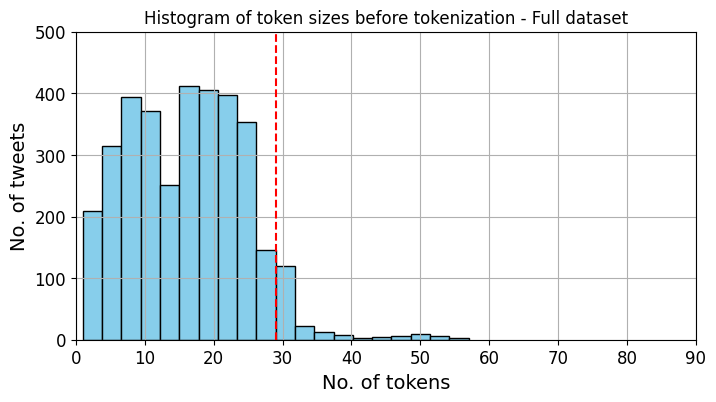
\includegraphics[width=\textwidth]{figures/token_hist.png}
        \caption{Before tokenization}
        \label{fig: token_hist}
    \end{subfigure}
    \hfill
    \begin{subfigure}[b]{0.48\textwidth}
        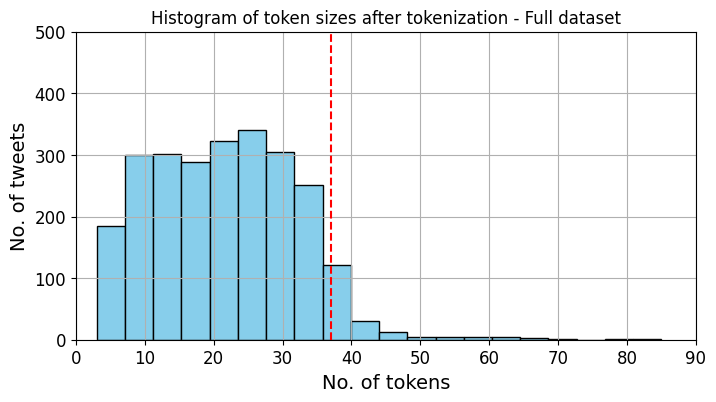
\includegraphics[width=\textwidth]{figures/token_pp_hist.png}
        \caption{After tokenization}
        \label{fig: token_pp_hist}
    \end{subfigure}
    \caption{The token count distribution for the full dataset of 3,449 tweets before and after tokenization with the red dashed line indicating 95\% coverage of tweets. BertTokenizer is used here.}
    \label{fig: bef_aft_token}
\end{figure}

The distribution of the number of tokens in the tweets from the pre-processed data from \cite{preotiuc-pietro_automatically_2019,jinModelingSeverityComplaints2021} before applying the model-specific tokenization is shown in Figure \ref{fig: token_hist}. Over 95\% of the tweets have 29 tokens or less. Using the BertTokenizer as an example, from Figure \ref{fig: token_pp_hist} it was found about 37 tokens are required to comprehensively cover 95\% of the tweets. The other tokenizers require between 35 and 43 tokens to cover the same percentage (refer Appendix \ref{sec: apdxa_token_dist}). This analysis assists in the decision on the appropriate \texttt{max\_value} for the tokenizer. A value of 50 ensures coverage of over 99\% of the tweets completely for all the tokenizers. This when used in conjunction with \texttt{truncation=True}, sets the maximum number of tokens for each input tweet to 50. Anything that follows is truncated and not used for training or inference. Additionally, since the dataset includes shorter tweets with resulting tokens less than 50, \texttt{padding} is set to \emph{'max\_length'} to apply padding up to 50 tokens.


\subsection{Tokenisation example}
An example tweet from the input data is shown in \textbf{A} below. The pre-processing applied by \cite{preotiuc-pietro_automatically_2019,jinModelingSeverityComplaints2021} results in punctuation as separate tokens, e.g. 'again' and '.'. The hashtags are retained as single tokens. After applying tokenisation using the \texttt{BertTokenizer}, the data is converted into a list of input IDs representing their reference into the model's vocabulary as shown in \textbf{B}. To better understand the effect of tokenization, \textbf{C} shows the decoded input from \textbf{B}. The tokenizer adds special tokens, \texttt{[CLS]} - classification token for the beginning of an input sequence, \texttt{[SEP]} - separator token to separate input sequences and \texttt{[PAD]} - padding token. Aside from this, punctuation is combined with the word for 'again.'. In the case of hashtags, the '\#' symbol has been separated out as a token.\\

\textbf{A - Tweet from input dataset}\newline

\begin{adjustbox}{minipage={\textwidth},fbox}
    \texttt{love it when i almost die rear ended by a semi cause my jeep turns off again
        . one day they will fix it \#jeepsucks \#chrysler}
\end{adjustbox} \newline\newline

\textbf{B - Encoding the input}\newline

\begin{adjustbox}{minipage={\textwidth},fbox}
    \texttt{[101, 2293, 2009, 2043, 1045, 2471, 3280, 4373, 3092, 2011, 1037, 4100, 3426,
                2026, 14007, 4332, 2125, 2153, 1012, 2028, 2154, 2027, 2097, 8081, 2009, 1001,
                14007, 6342, 10603, 1001, 17714, 102, 0, 0, 0, 0, 0, 0, 0, 0, 0, 0, 0, 0, 0,
                0, 0, 0, 0, 0]}
\end{adjustbox} \newline\newline

\textbf{C - Decoding the tokenized input}\newline

\begin{adjustbox}{minipage={\textwidth},fbox}
    \texttt{[CLS] love it when i almost die rear ended by a semi cause my jeep turns off
        again. one day they will fix it \# jeepsucks \# chrysler [SEP] [PAD] [PAD] [PAD]
            [PAD] [PAD] [PAD] [PAD] [PAD] [PAD] [PAD] [PAD] [PAD] [PAD] [PAD] [PAD] [PAD]
            [PAD] [PAD]}
\end{adjustbox}\\ \\

\section{Experiment set 1: Predictive performance comparison of BERT variants}
In the first experiment, the objective is to identify which of the models performs the best for the text classification task of complaint identification. Additionally, the relative performance of the models and the inference time will be analysed to assess how the model size impacts these aspects. A nested cross-validation approach will be used to experiment finetuning the model with various learning rate hyperparameter values and calculate mean performance metrics on inference. All models in scope for the experiments are pre-trained, hence finetuning will be performed for the downstream complaints identification task.\\

The nested cross-validation approach utilized is adapted from \cite{preotiuc-pietro_automatically_2019}. The outer loop consists of 6 iterations and the inner loop of 4 iterations. Each outer loop includes a stratified split of the entire dataset into train (\textbf{a}) and test (\textbf{b}) datasets. Within the inner loop, \textbf{a} is further split into inner train and dev datasets using stratified split with each iteration, finetuning and validating on 1 of the 4 learning rates set for hyperparameter tuning. The best model from the inner loop is selected based on the F1 score on the dev dataset. This best model is used to perform inference using the test dataset, \textbf{b}. At the end of the 6 outer loop iterations, the mean of the performance metrics is calculated as the final metrics for that model. While \cite{preotiuc-pietro_automatically_2019} used 10 iterations for the outer loop, it has been restricted to 6 for the experiments considering significant variations were not observed on the metrics. This is likely due to the smaller size of the dataset and 6 stratified splits capturing sufficient variability in the input dataset.\\
\begin{table}[ht]
    \captionsetup{font=small}
    \small
    \centering
    \begin{tabularx}{\textwidth}{|X|c|}
        \hline
        \rowcolor[gray]{0.7}
        \textbf{Parameter}        & \textbf{Value}           \\
        \hline
        Outer loop iterations     & 6                        \\
        \rowcolor[gray]{0.9}
        Inner loop iterations     & 4                        \\
        Random Seed               & 2023                     \\
        \hline
        \hline
        \rowcolor[gray]{0.7}
        \textbf{Hyperparameter}   & \textbf{Value}           \\
        \hline
        No. of Epochs             & 4                        \\
        \rowcolor[gray]{0.9}
        Learning Rate             & [1e-5, 5e-6, 5e-5, 3e-5] \\
        All other hyperparameters & Model defaults           \\
        \hline
    \end{tabularx}
    \caption{The choice of key parameters and hyperparameters used for experiment set 1.}
    \label{tab: exp1_params}
\end{table}

The key choices for the experiments including that of the hyperparameters are described in Table \ref{tab: exp1_params}. For the stratified split, the \texttt{StratifiedKFold} function from \texttt{sklearn} library is used. This results in approximately 2874 and 575 tweets for the outer loop's train and test datasets and 2155 and 719 tweets for the inner loop's train and dev datasets. The number of epochs is set to 4 in line with official documentation for BERT\footnote{\url{https://github.com/google-research/bert}} where they use between 2 and 4 epochs for the various downstream tasks. The learning rate includes the default rate used by the models as well as a range of alternate values. All other hyperparameters take on their default values for the models as defined in the \texttt{transformers} library.\\

For the predictive performance metrics, precision, recall, accuracy, F1 and Area under the ROC Curve (AUC) scores are computed for both the inner loop's validation as well as the outer loop's testing. Further, the final metrics for each model are based on each of the mean metrics from the 6 outer loop iterations. Additionally, the samples per second and steps per second are captured for each of the models during the inference phase to analyse the time taken for inference in relation to the model size.

\section{Experiment set 2: Cross-domain predictive performance comparison}
Cross-domain experiments are conducted to understand how the performance of finetuned models varies as the volume, domain and class balance of the tweets change.  This approach also offers an avenue to assess any linguistic variations among complaints across different domains and their consequent effects on the classification performance. \\

For the experiments, the best-performing model from the first experiment is utilised. The tweets for each of the 9 domains are used for training separately with tweets from every other domain used for testing. Additionally, each domain is used for testing while training is based on all tweets except the domain used for testing. Stratified split is applied on the training dataset for each domain using the \texttt{StratifiedKFold} function from \texttt{sklearn} library for 3 iterations of finetuning. At the end of each iteration, inference is performed on the testing data.  The number of epochs remains at '4', similar to experiment set 1 while the learning rate used is the best learning for the selected model from experiment set 1. All other hyperparameters are the model defaults. The parameters and hyperparameters used for the experiment are listed in Table \ref{tab: exp2_params}.\\

In this set of experiments, only the most effective model identified from the previous experiment is utilised. The model is finetuned using tweets belonging to one domain at a time while testing is performed for each of the remaining domains separately and performance recorded. Additionally, each domain is tested on a  model which is finetuned on all tweets except the domain used for testing.\\

To ensure the balance of classes is maintained for the training and evaluation sets, a stratified split is applied using the \texttt{StratifiedKFold} function from the \texttt{sklearn} library. This process is repeated for three iterations of finetuning. Following each iteration, the model's performance is evaluated through inference on the testing data. The experiment maintains a consistent number of epochs of 4, similar to the first experiment. The learning rate is determined by the optimal value identified in the initial experiment for the selected model. All other hyperparameters follow the model's default settings. For details of the parameters and hyperparameters employed in this experiment, please refer to Table \ref{tab: exp2_params}.

\begin{table}[ht]
    \captionsetup{font=small}
    \small
    \centering
    \begin{tabularx}{\textwidth}{|X|c|}
        \hline
        \rowcolor[gray]{0.7}
        \textbf{Parameter}        & \textbf{Value}                       \\
        \hline
        No. of iterations         & 3                                    \\
        \rowcolor[gray]{0.9}
        Random Seed               & 2023                                 \\
        \hline
        \hline
        \rowcolor[gray]{0.7}
        \textbf{Hyperparameter}   & \textbf{Value}                       \\
        \hline
        No. of Epochs             & 4                                    \\
        \rowcolor[gray]{0.9}
        Learning Rate             & Best learning rate from experiment set 1 \\
        All other hyperparameters & Model defaults                       \\
        \hline
    \end{tabularx}
    \caption{The choice of key parameters and hyperparameters used for experiment set 2. Refer to the Chapter on results for the model and learning rate used for this experiment. }
    \label{tab: exp2_params}
\end{table}
For each iteration and combination of domains for finetuning and testing, the prediction performance metrics are calculated for precision, recall, accuracy, F1, and AUC. At the end of the third iteration, the mean of the metrics is calculated. The results and findings from this set of experiments are presented in Chapter 4.

\section{Ethical, Professional and Legal Issues}
The data used for the experiments were created by \cite{preotiuc-pietro_automatically_2019} and further enhanced with complaints severity type annotation by \cite{jinModelingSeverityComplaints2021}. This data is anonymised and is available in the public domain\footnote{\url{ https://archive.org/details/complaint_severity_data}}. No additional data has been collected for the experiments conducted for this project. To ensure the appropriate compliance with the ethical review requirements of the University of Sheffield, a self-declared ethics review application with reference number 054854 was raised and subsequently approved by the University Research Ethics Committee.
